% Options for packages loaded elsewhere
\PassOptionsToPackage{unicode}{hyperref}
\PassOptionsToPackage{hyphens}{url}
\PassOptionsToPackage{dvipsnames,svgnames,x11names}{xcolor}
%
\documentclass[
  letterpaper,
  DIV=11,
  numbers=noendperiod]{scrartcl}

\usepackage{amsmath,amssymb}
\usepackage{iftex}
\ifPDFTeX
  \usepackage[T1]{fontenc}
  \usepackage[utf8]{inputenc}
  \usepackage{textcomp} % provide euro and other symbols
\else % if luatex or xetex
  \usepackage{unicode-math}
  \defaultfontfeatures{Scale=MatchLowercase}
  \defaultfontfeatures[\rmfamily]{Ligatures=TeX,Scale=1}
\fi
\usepackage{lmodern}
\ifPDFTeX\else  
    % xetex/luatex font selection
\fi
% Use upquote if available, for straight quotes in verbatim environments
\IfFileExists{upquote.sty}{\usepackage{upquote}}{}
\IfFileExists{microtype.sty}{% use microtype if available
  \usepackage[]{microtype}
  \UseMicrotypeSet[protrusion]{basicmath} % disable protrusion for tt fonts
}{}
\makeatletter
\@ifundefined{KOMAClassName}{% if non-KOMA class
  \IfFileExists{parskip.sty}{%
    \usepackage{parskip}
  }{% else
    \setlength{\parindent}{0pt}
    \setlength{\parskip}{6pt plus 2pt minus 1pt}}
}{% if KOMA class
  \KOMAoptions{parskip=half}}
\makeatother
\usepackage{xcolor}
\setlength{\emergencystretch}{3em} % prevent overfull lines
\setcounter{secnumdepth}{5}
% Make \paragraph and \subparagraph free-standing
\makeatletter
\ifx\paragraph\undefined\else
  \let\oldparagraph\paragraph
  \renewcommand{\paragraph}{
    \@ifstar
      \xxxParagraphStar
      \xxxParagraphNoStar
  }
  \newcommand{\xxxParagraphStar}[1]{\oldparagraph*{#1}\mbox{}}
  \newcommand{\xxxParagraphNoStar}[1]{\oldparagraph{#1}\mbox{}}
\fi
\ifx\subparagraph\undefined\else
  \let\oldsubparagraph\subparagraph
  \renewcommand{\subparagraph}{
    \@ifstar
      \xxxSubParagraphStar
      \xxxSubParagraphNoStar
  }
  \newcommand{\xxxSubParagraphStar}[1]{\oldsubparagraph*{#1}\mbox{}}
  \newcommand{\xxxSubParagraphNoStar}[1]{\oldsubparagraph{#1}\mbox{}}
\fi
\makeatother

\usepackage{color}
\usepackage{fancyvrb}
\newcommand{\VerbBar}{|}
\newcommand{\VERB}{\Verb[commandchars=\\\{\}]}
\DefineVerbatimEnvironment{Highlighting}{Verbatim}{commandchars=\\\{\}}
% Add ',fontsize=\small' for more characters per line
\usepackage{framed}
\definecolor{shadecolor}{RGB}{241,243,245}
\newenvironment{Shaded}{\begin{snugshade}}{\end{snugshade}}
\newcommand{\AlertTok}[1]{\textcolor[rgb]{0.68,0.00,0.00}{#1}}
\newcommand{\AnnotationTok}[1]{\textcolor[rgb]{0.37,0.37,0.37}{#1}}
\newcommand{\AttributeTok}[1]{\textcolor[rgb]{0.40,0.45,0.13}{#1}}
\newcommand{\BaseNTok}[1]{\textcolor[rgb]{0.68,0.00,0.00}{#1}}
\newcommand{\BuiltInTok}[1]{\textcolor[rgb]{0.00,0.23,0.31}{#1}}
\newcommand{\CharTok}[1]{\textcolor[rgb]{0.13,0.47,0.30}{#1}}
\newcommand{\CommentTok}[1]{\textcolor[rgb]{0.37,0.37,0.37}{#1}}
\newcommand{\CommentVarTok}[1]{\textcolor[rgb]{0.37,0.37,0.37}{\textit{#1}}}
\newcommand{\ConstantTok}[1]{\textcolor[rgb]{0.56,0.35,0.01}{#1}}
\newcommand{\ControlFlowTok}[1]{\textcolor[rgb]{0.00,0.23,0.31}{\textbf{#1}}}
\newcommand{\DataTypeTok}[1]{\textcolor[rgb]{0.68,0.00,0.00}{#1}}
\newcommand{\DecValTok}[1]{\textcolor[rgb]{0.68,0.00,0.00}{#1}}
\newcommand{\DocumentationTok}[1]{\textcolor[rgb]{0.37,0.37,0.37}{\textit{#1}}}
\newcommand{\ErrorTok}[1]{\textcolor[rgb]{0.68,0.00,0.00}{#1}}
\newcommand{\ExtensionTok}[1]{\textcolor[rgb]{0.00,0.23,0.31}{#1}}
\newcommand{\FloatTok}[1]{\textcolor[rgb]{0.68,0.00,0.00}{#1}}
\newcommand{\FunctionTok}[1]{\textcolor[rgb]{0.28,0.35,0.67}{#1}}
\newcommand{\ImportTok}[1]{\textcolor[rgb]{0.00,0.46,0.62}{#1}}
\newcommand{\InformationTok}[1]{\textcolor[rgb]{0.37,0.37,0.37}{#1}}
\newcommand{\KeywordTok}[1]{\textcolor[rgb]{0.00,0.23,0.31}{\textbf{#1}}}
\newcommand{\NormalTok}[1]{\textcolor[rgb]{0.00,0.23,0.31}{#1}}
\newcommand{\OperatorTok}[1]{\textcolor[rgb]{0.37,0.37,0.37}{#1}}
\newcommand{\OtherTok}[1]{\textcolor[rgb]{0.00,0.23,0.31}{#1}}
\newcommand{\PreprocessorTok}[1]{\textcolor[rgb]{0.68,0.00,0.00}{#1}}
\newcommand{\RegionMarkerTok}[1]{\textcolor[rgb]{0.00,0.23,0.31}{#1}}
\newcommand{\SpecialCharTok}[1]{\textcolor[rgb]{0.37,0.37,0.37}{#1}}
\newcommand{\SpecialStringTok}[1]{\textcolor[rgb]{0.13,0.47,0.30}{#1}}
\newcommand{\StringTok}[1]{\textcolor[rgb]{0.13,0.47,0.30}{#1}}
\newcommand{\VariableTok}[1]{\textcolor[rgb]{0.07,0.07,0.07}{#1}}
\newcommand{\VerbatimStringTok}[1]{\textcolor[rgb]{0.13,0.47,0.30}{#1}}
\newcommand{\WarningTok}[1]{\textcolor[rgb]{0.37,0.37,0.37}{\textit{#1}}}

\providecommand{\tightlist}{%
  \setlength{\itemsep}{0pt}\setlength{\parskip}{0pt}}\usepackage{longtable,booktabs,array}
\usepackage{calc} % for calculating minipage widths
% Correct order of tables after \paragraph or \subparagraph
\usepackage{etoolbox}
\makeatletter
\patchcmd\longtable{\par}{\if@noskipsec\mbox{}\fi\par}{}{}
\makeatother
% Allow footnotes in longtable head/foot
\IfFileExists{footnotehyper.sty}{\usepackage{footnotehyper}}{\usepackage{footnote}}
\makesavenoteenv{longtable}
\usepackage{graphicx}
\makeatletter
\def\maxwidth{\ifdim\Gin@nat@width>\linewidth\linewidth\else\Gin@nat@width\fi}
\def\maxheight{\ifdim\Gin@nat@height>\textheight\textheight\else\Gin@nat@height\fi}
\makeatother
% Scale images if necessary, so that they will not overflow the page
% margins by default, and it is still possible to overwrite the defaults
% using explicit options in \includegraphics[width, height, ...]{}
\setkeys{Gin}{width=\maxwidth,height=\maxheight,keepaspectratio}
% Set default figure placement to htbp
\makeatletter
\def\fps@figure{htbp}
\makeatother

\KOMAoption{captions}{tableheading}
\makeatletter
\@ifpackageloaded{caption}{}{\usepackage{caption}}
\AtBeginDocument{%
\ifdefined\contentsname
  \renewcommand*\contentsname{Table of contents}
\else
  \newcommand\contentsname{Table of contents}
\fi
\ifdefined\listfigurename
  \renewcommand*\listfigurename{List of Figures}
\else
  \newcommand\listfigurename{List of Figures}
\fi
\ifdefined\listtablename
  \renewcommand*\listtablename{List of Tables}
\else
  \newcommand\listtablename{List of Tables}
\fi
\ifdefined\figurename
  \renewcommand*\figurename{Figure}
\else
  \newcommand\figurename{Figure}
\fi
\ifdefined\tablename
  \renewcommand*\tablename{Table}
\else
  \newcommand\tablename{Table}
\fi
}
\@ifpackageloaded{float}{}{\usepackage{float}}
\floatstyle{ruled}
\@ifundefined{c@chapter}{\newfloat{codelisting}{h}{lop}}{\newfloat{codelisting}{h}{lop}[chapter]}
\floatname{codelisting}{Listing}
\newcommand*\listoflistings{\listof{codelisting}{List of Listings}}
\makeatother
\makeatletter
\makeatother
\makeatletter
\@ifpackageloaded{caption}{}{\usepackage{caption}}
\@ifpackageloaded{subcaption}{}{\usepackage{subcaption}}
\makeatother

\ifLuaTeX
  \usepackage{selnolig}  % disable illegal ligatures
\fi
\usepackage{bookmark}

\IfFileExists{xurl.sty}{\usepackage{xurl}}{} % add URL line breaks if available
\urlstyle{same} % disable monospaced font for URLs
\hypersetup{
  pdftitle={Biostat 212A Homework 3},
  pdfauthor={Jiaye Tian and UID: 306541095},
  colorlinks=true,
  linkcolor={blue},
  filecolor={Maroon},
  citecolor={Blue},
  urlcolor={Blue},
  pdfcreator={LaTeX via pandoc}}


\title{Biostat 212A Homework 3}
\usepackage{etoolbox}
\makeatletter
\providecommand{\subtitle}[1]{% add subtitle to \maketitle
  \apptocmd{\@title}{\par {\large #1 \par}}{}{}
}
\makeatother
\subtitle{Due Feb 18, 2025 @ 11:59PM}
\author{Jiaye Tian and UID: 306541095}
\date{2025-02-19}

\begin{document}
\maketitle

\renewcommand*\contentsname{Table of contents}
{
\hypersetup{linkcolor=}
\setcounter{tocdepth}{4}
\tableofcontents
}

\subsection{ISL Exercise 5.4.2 (10pts)}\label{isl-exercise-5.4.2-10pts}

We will now derive the probability that a given observation is part of a
bootstrap sample. Suppose that we obtain a bootstrap sample from a set
of n observations.

\textbf{(a)}\\
\(1 - 1/n\)\\
The probability that the 𝑗th observation is not the first bootstrap
observation is 1 - 1/n. Since there are n observations, each has an
equal probability of 1/n of being chosen first. Therefore, the
probability that the jth observation is not selected as the first
bootstrap observation is 1 − 1/n.

\textbf{(b)}\\
\(1 - 1/n\)\\
Since each bootstrap observation is independently drawn with
replacement, every selection follows the same probability distribution.

\textbf{(c)} In bootstrapping, each sample is drawn independently with
replacement from the original dataset of size n.~The probability that
the jth observation is not chosen in a single draw is 1−1/n.~Since we
draw n times independently, the probability that it never appears in the
bootstrap sample is \[
(1 - \frac{1}{n}) \cdots (1 - \frac{1}{n}) = (1 - \frac{1}{n})^n
\]

\textbf{(d)}\\
When n = 5, the probability that the jth observation appears in the
bootstrap sample is
\(P(\text{jth obs in bootstrap sample when n=5}) = 1 - (1 - \frac{1}{5})^5 = 0.672.\)

\textbf{(e)}\\
When n = 100, the probability that the jth observation appears in the
bootstrap sample is
\(P(\text{jth obs in bootstrap sample when n=100}) = 1 - (1 - 1/100)^{100} = 0.634.\)

\textbf{(f)} When n = 1000, the probability that the jth observation
appears in the bootstrap sample is
\(P(\text{jth obs in bootstrap sample when n=1000}) = 1 - (1 - \frac{1}{1000})^{1000} = 0.632.\)

\textbf{(g)}

\begin{Shaded}
\begin{Highlighting}[]
\NormalTok{n }\OtherTok{\textless{}{-}} \FunctionTok{seq}\NormalTok{(}\DecValTok{1}\NormalTok{, }\DecValTok{100000}\NormalTok{, }\AttributeTok{by=}\DecValTok{10}\NormalTok{)}

\NormalTok{prob }\OtherTok{\textless{}{-}} \DecValTok{1} \SpecialCharTok{{-}}\NormalTok{ (}\DecValTok{1} \SpecialCharTok{{-}} \DecValTok{1}\SpecialCharTok{/}\NormalTok{n)}\SpecialCharTok{\^{}}\NormalTok{n}

\NormalTok{asymptote }\OtherTok{\textless{}{-}} \DecValTok{1} \SpecialCharTok{{-}} \DecValTok{1}\SpecialCharTok{/}\FunctionTok{exp}\NormalTok{(}\DecValTok{1}\NormalTok{)}

\NormalTok{asymptote}
\end{Highlighting}
\end{Shaded}

\begin{verbatim}
[1] 0.6321206
\end{verbatim}

\begin{Shaded}
\begin{Highlighting}[]
\FunctionTok{plot}\NormalTok{(n, prob, }\AttributeTok{type=}\StringTok{"l"}\NormalTok{, }\AttributeTok{log=}\StringTok{"x"}\NormalTok{, }
     \AttributeTok{xlab=}\StringTok{"n (log scale)"}\NormalTok{, }\AttributeTok{ylab=}\StringTok{"Probability of inclusion"}\NormalTok{,}
     \AttributeTok{main=}\StringTok{"Probability of an Observation in a Bootstrap Sample"}\NormalTok{)}

\FunctionTok{abline}\NormalTok{(}\AttributeTok{h=}\DecValTok{1} \SpecialCharTok{{-}} \DecValTok{1}\SpecialCharTok{/}\FunctionTok{exp}\NormalTok{(}\DecValTok{1}\NormalTok{), }\AttributeTok{col=}\StringTok{"red"}\NormalTok{, }\AttributeTok{lty=}\DecValTok{2}\NormalTok{)}
\end{Highlighting}
\end{Shaded}

\begin{center}
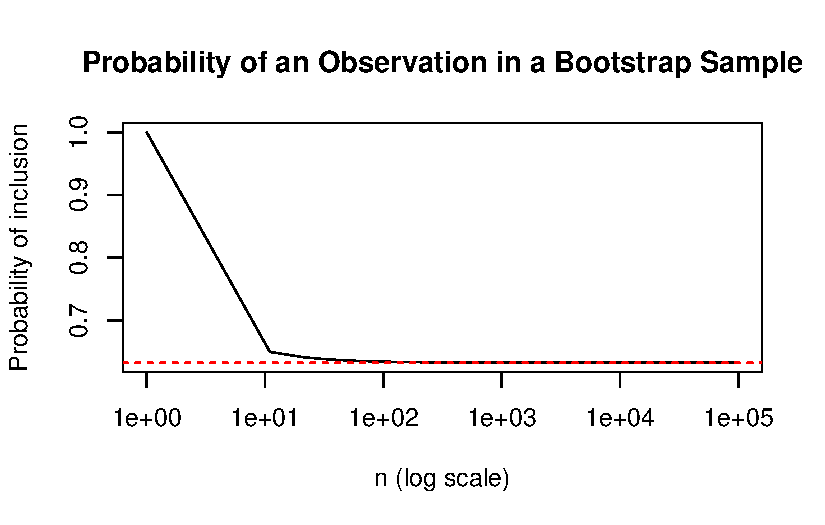
\includegraphics{hw3_files/figure-pdf/unnamed-chunk-1-1.pdf}
\end{center}

\textbf{(h)}

\begin{Shaded}
\begin{Highlighting}[]
\NormalTok{contains\_j }\OtherTok{\textless{}{-}} \FunctionTok{rep}\NormalTok{(}\ConstantTok{NA}\NormalTok{, }\DecValTok{10000}\NormalTok{)}
\ControlFlowTok{for}\NormalTok{ (i }\ControlFlowTok{in} \DecValTok{1}\SpecialCharTok{:}\DecValTok{10000}\NormalTok{) \{}
\NormalTok{    contains\_j[i] }\OtherTok{\textless{}{-}} \FunctionTok{sum}\NormalTok{(}\FunctionTok{sample}\NormalTok{(}\DecValTok{1}\SpecialCharTok{:}\DecValTok{100}\NormalTok{, }\AttributeTok{rep =} \ConstantTok{TRUE}\NormalTok{) }\SpecialCharTok{==} \DecValTok{4}\NormalTok{) }\SpecialCharTok{\textgreater{}} \DecValTok{0}
\NormalTok{\}}
\FunctionTok{mean}\NormalTok{(contains\_j)}
\end{Highlighting}
\end{Shaded}

\begin{verbatim}
[1] 0.6316
\end{verbatim}

From calculus, we know:

\[
\lim_{n\rightarrow\infty}\left(1 - \frac{1}{n}\right)^n = \frac{1}{e}.
\]

Thus, the probability that a bootstrap sample of size ( n ) contains the
( j )th observation is:

\[
P(\text{included}) = 1 - \left(1 - \frac{1}{n}\right)^n.
\]

Taking the limit as ( n \to \infty ):

\[
\lim_{n \to \infty} P(\text{included}) = 1 - \frac{1}{e} \approx 0.632.
\]

So for large ( n ), each observation appears in the bootstrap sample
about \textbf{63.2\%} of the time.

\subsection{ISL Exercise 5.4.9 (20pts)}\label{isl-exercise-5.4.9-20pts}

\begin{Shaded}
\begin{Highlighting}[]
\FunctionTok{library}\NormalTok{(MASS)}
\FunctionTok{library}\NormalTok{(boot)}
\FunctionTok{attach}\NormalTok{(Boston)}
\end{Highlighting}
\end{Shaded}

\begin{Shaded}
\begin{Highlighting}[]
\NormalTok{mu.hat }\OtherTok{\textless{}{-}} \FunctionTok{mean}\NormalTok{(medv)}
\NormalTok{mu.hat}
\end{Highlighting}
\end{Shaded}

\begin{verbatim}
[1] 22.53281
\end{verbatim}

\textbf{(b)}

\begin{Shaded}
\begin{Highlighting}[]
\NormalTok{se.hat }\OtherTok{\textless{}{-}} \FunctionTok{sd}\NormalTok{(medv) }\SpecialCharTok{/} \FunctionTok{sqrt}\NormalTok{(}\FunctionTok{dim}\NormalTok{(Boston)[}\DecValTok{1}\NormalTok{])}
\NormalTok{se.hat}
\end{Highlighting}
\end{Shaded}

\begin{verbatim}
[1] 0.4088611
\end{verbatim}

\textbf{(c)}

\begin{Shaded}
\begin{Highlighting}[]
\FunctionTok{set.seed}\NormalTok{(}\DecValTok{1}\NormalTok{)}
\NormalTok{boot.fn }\OtherTok{\textless{}{-}} \ControlFlowTok{function}\NormalTok{(data, index) \{}
\NormalTok{    mu }\OtherTok{\textless{}{-}} \FunctionTok{mean}\NormalTok{(data[index])}
    \FunctionTok{return}\NormalTok{ (mu)}
\NormalTok{\}}
\FunctionTok{boot}\NormalTok{(medv, boot.fn, }\DecValTok{1000}\NormalTok{)}
\end{Highlighting}
\end{Shaded}

\begin{verbatim}

ORDINARY NONPARAMETRIC BOOTSTRAP


Call:
boot(data = medv, statistic = boot.fn, R = 1000)


Bootstrap Statistics :
    original      bias    std. error
t1* 22.53281 0.007650791   0.4106622
\end{verbatim}

\textbf{(d)}

\begin{Shaded}
\begin{Highlighting}[]
\FunctionTok{t.test}\NormalTok{(medv)}
\end{Highlighting}
\end{Shaded}

\begin{verbatim}

    One Sample t-test

data:  medv
t = 55.111, df = 505, p-value < 2.2e-16
alternative hypothesis: true mean is not equal to 0
95 percent confidence interval:
 21.72953 23.33608
sample estimates:
mean of x 
 22.53281 
\end{verbatim}

\textbf{(e)}

\begin{Shaded}
\begin{Highlighting}[]
\NormalTok{med.hat }\OtherTok{\textless{}{-}} \FunctionTok{median}\NormalTok{(medv)}
\NormalTok{med.hat}
\end{Highlighting}
\end{Shaded}

\begin{verbatim}
[1] 21.2
\end{verbatim}

\textbf{(f)}

\begin{Shaded}
\begin{Highlighting}[]
\NormalTok{boot.fn }\OtherTok{\textless{}{-}} \ControlFlowTok{function}\NormalTok{(data, index) \{}
\NormalTok{    mu }\OtherTok{\textless{}{-}} \FunctionTok{median}\NormalTok{(data[index])}
    \FunctionTok{return}\NormalTok{ (mu)}
\NormalTok{\}}
\FunctionTok{boot}\NormalTok{(medv, boot.fn, }\DecValTok{1000}\NormalTok{)}
\end{Highlighting}
\end{Shaded}

\begin{verbatim}

ORDINARY NONPARAMETRIC BOOTSTRAP


Call:
boot(data = medv, statistic = boot.fn, R = 1000)


Bootstrap Statistics :
    original  bias    std. error
t1*     21.2 -0.0386   0.3770241
\end{verbatim}

We get an estimated median value of 21.2 which is equal to the value got
in (e), with a standard error of 0.3874 which is relatively small
compared to median value.

\textbf{(g)}

\begin{Shaded}
\begin{Highlighting}[]
\NormalTok{percent.hat }\OtherTok{\textless{}{-}} \FunctionTok{quantile}\NormalTok{(medv, }\FunctionTok{c}\NormalTok{(}\FloatTok{0.1}\NormalTok{))}
\NormalTok{percent.hat}
\end{Highlighting}
\end{Shaded}

\begin{verbatim}
  10% 
12.75 
\end{verbatim}

\textbf{(h)}

\begin{Shaded}
\begin{Highlighting}[]
\NormalTok{boot.fn }\OtherTok{\textless{}{-}} \ControlFlowTok{function}\NormalTok{(data, index) \{}
\NormalTok{    mu }\OtherTok{\textless{}{-}} \FunctionTok{quantile}\NormalTok{(data[index], }\FunctionTok{c}\NormalTok{(}\FloatTok{0.1}\NormalTok{))}
    \FunctionTok{return}\NormalTok{ (mu)}
\NormalTok{\}}
\FunctionTok{boot}\NormalTok{(medv, boot.fn, }\DecValTok{1000}\NormalTok{)}
\end{Highlighting}
\end{Shaded}

\begin{verbatim}

ORDINARY NONPARAMETRIC BOOTSTRAP


Call:
boot(data = medv, statistic = boot.fn, R = 1000)


Bootstrap Statistics :
    original  bias    std. error
t1*    12.75  0.0186   0.4925766
\end{verbatim}

We get an estimated tenth percentile value of 12.75 which is again equal
to the value obtained in (g), with a standard error of 0.5113 which is
relatively small compared to percentile value.

\subsection{Least squares is MLE
(10pts)}\label{least-squares-is-mle-10pts}

Show that in the case of linear model with Gaussian errors, maximum
likelihood and least squares are the same thing, and \(C_p\) and AIC are
equivalent.

To show that least squares and maximum likelihood estimation (MLE) are
equivalent, consider the linear model:

\[
Y = X\beta + \varepsilon, \quad \varepsilon \sim \mathcal{N}(0, \sigma^2 I).
\]

The likelihood function for ( Y ) is:

\[
L(\beta, \sigma^2) = \frac{1}{(2\pi\sigma^2)^{n/2}} \exp\left( -\frac{1}{2\sigma^2} \| Y - X\beta \|^2 \right).
\]

Taking the log:

\[
\log L(\beta, \sigma^2) = -\frac{n}{2} \log (2\pi\sigma^2) - \frac{1}{2\sigma^2} \| Y - X\beta \|^2.
\]

Maximizing ( L ) with respect to ( \beta ) is equivalent to minimizing:

\[
\| Y - X\beta \|^2.
\]

which is exactly the least squares objective function. Therefore, the
OLS estimator is the same as the MLE estimator:

\[
\hat{\beta}_{\text{MLE}} = \hat{\beta}_{\text{OLS}} = (X^T X)^{-1} X^T Y.
\]

Thus, we have shown that least squares and MLE are the same in the
Gaussian setting.

\begin{center}\rule{0.5\linewidth}{0.5pt}\end{center}

Mallows' ( C\_p ) is defined as:

\[
C_p = \frac{1}{n} (RSS + 2d\hat{\sigma}^2),
\] - ( RSS ) is the \textbf{residual sum of squares},\\
- ( d ) is the \textbf{number of parameters},\\
- hat\{\sigma\}\^{}2 is an estimate of the error variance.

The AIC is:

\[
AIC = -2 \log L + 2d.
\]

Since:

\[
-2 \log L \approx n \log (RSS/n) + \text{constant},
\]

it follows that:

\[
AIC \approx C_p.
\]

Thus, in the Gaussian setting, ( C\_p ) and AIC are equivalent in model
selection.

\subsection{ISL Exercise 6.6.1 (10pts)}\label{isl-exercise-6.6.1-10pts}

\textbf{(a)}\\
When performing best subset selection, the model with \(k\) predictors
is chosen from all \(C_p^k\) possible models with \(k\) predictors,
selecting the one with the \textbf{smallest residual sum of squares
(RSS)}.

In \textbf{forward stepwise selection}, the model with \(k\) predictors
is selected from the \(p - k + 1\) models that result from adding one
predictor to the best \(\mathcal{M}_{k - 1}\)-predictor model.

In \textbf{backward stepwise selection}, the model with \(k\) predictors
is selected from the \(k + 1\) models that result from removing one
predictor from the best \(\mathcal{M}_{k + 1}\)-predictor model.

Since best subset selection considers all possible models at each step,
it always finds the model with the \textbf{lowest training RSS}, making
it the most optimal approach in terms of training error.

\textbf{(b)}\\
The model selected by best subset selection has the smallest training
RSS because it evaluates all possible models with k predictors and
chooses the one with the lowest residual sum of squares (RSS). In
contrast, forward stepwise selection and backward stepwise selection
only explore a subset of possible models, meaning they may not always
find the model with the lowest RSS. However, in some cases, all three
methods might end up selecting the same model.

\textbf{(c) True or False:}\\
- \textbf{\emph{i}} True.\\
- \textbf{\emph{ii}} True.\\
- \textbf{\emph{iii}} False.\\
- \textbf{\emph{iv}} False.\\
- \textbf{\emph{v}} False.

\subsection{ISL Exercise 6.6.3 (10pts)}\label{isl-exercise-6.6.3-10pts}

\textbf{(a)}

\begin{quote}
\textbf{Part iv - The training RSS steadily decreases as ( s )
increases.}
\end{quote}

LASSO regression constrains the sum of absolute values of the
coefficients: \(\sum_{j=1}^{p} |\beta_j| \leq s\) where \(s\) controls
the degree of regularization.

As \(s\) increases, the constraint loosens, allowing the coefficients
\(\beta_j\) to move closer to their least squares estimates. This
increases model flexibility and leads to a reduction in training RSS.

When \(s\) becomes sufficiently large, the constraint no longer affects
the solution, meaning the estimated coefficients minimize:
\(RSS = \sum_{i=1}^{n} \left( y_i - \beta_0 - \sum_{j=1}^{p} \beta_j x_{ij} \right)^2\)
and match the ordinary least squares (OLS) estimates. Up to this point,
the training RSS decreases monotonically as \(s\) increases.

\textbf{(b)}

\begin{quote}
\textbf{Part ii - Decrease initially, then eventually increase in a U
shape.}
\end{quote}

When \(s = 0\), the only \(\hat{\beta}\) that satisfies
\(\sum_{j=1}^{p} |\beta_j| \leq s\) is the zero vector, meaning the
model simply predicts the mean \(\hat{y} = \bar{y}\), leading to a very
high test RSS.

As \(s\) increases, the restriction loosens, allowing the coefficients
\(\beta_j\) to take on nonzero values. This increases the model's
flexibility, enabling it to fit the data better and initially decreasing
the test RSS.

However, as \(s\) continues to increase, the model becomes overly
complex, fitting noise in the training data and leading to overfitting.
At this stage, test RSS starts rising again, forming a characteristic
U-shaped pattern.

\textbf{(c)}

\begin{quote}
\textbf{Part ii - Steadily increase.}
\end{quote}

As \(s\) increases from zero, the constraint region expands, effectively
reducing \(\lambda\) (shrinkage). This increases model flexibility,
leading to a steady rise in variance. If \(s\) becomes large enough that
\(\hat{\beta}\) falls within the unconstrained region, variance
stabilizes, as the selected \(\hat{\beta}\) aligns with the least
squares estimate.

\textbf{(d)}

\begin{quote}
\textbf{Part iv - Steadily Decrease.}
\end{quote}

Similar to part (c), increasing model flexibility reduces bias. As \(s\)
gets larger, constraints loosen, coefficients adjust, and bias is
reduced. But as soon as the least squares solution lies inside the
constraint region, bias reduction ceases.

\textbf{(e)}

\begin{quote}
\textbf{Part v. - Remain Constant.}
\end{quote}

The irreducible error arises from inherent uncertainty or noise in the
system. It is invariant to model flexibility since there are some
explanatory variables may be unmeasured or certain variations in \(y\)
cannot be measured by \(X\). Thus, no matter how well the model is
specified, the irreducible error is entirely independent of \(s\).

\[
\text{Irreducible Error} = \mathbb{E}[(y - f(X))^2]
\]

\subsection{ISL Exercise 6.6.4 (10pts)}\label{isl-exercise-6.6.4-10pts}

\textbf{(a)}

\begin{quote}
\textbf{Part iii - Steadily Increase.}
\end{quote}

When \(\lambda = 0\), ridge regression estimates \(\hat{\beta}\) as the
least squares solution, since the penalty term is absent. This provides
the lowest possible training RSS. As \(\lambda\) increases, the penalty
term introduces shrinkage, which decreases the values of \(\beta_j\)
coefficients. This constraint limits model flexibility, preventing it
from fitting the training data as closely. Consequently, the training
RSS steadily increases as \(\lambda\) grows.

\textbf{(b)}

\begin{quote}
\textbf{Part ii - Decrease initially, then eventually increase in a U
shape.}
\end{quote}

As \(\lambda\) (shrinkage) increases, variance is reduced, which
initially outweighs the cost of shrinking \(\hat{\beta}\) coefficients
towards zero. As a result, the test RSS decreases. When \(\\\\lambda\)
continues to grow, though, over-shrinkage produces underfitting,
reducing predictive performance. At this point, the increased bias
outweighs the reduced variance, causing test RSS to rise again, forming
a characteristic U-shaped pattern.

\textbf{(c)}

\begin{quote}
\textbf{Part iv - Steadily Decrease.}
\end{quote}

As \(\lambda\) increases, model flexibility decreases since the
\(\beta\) coefficients become smaller in magnitude and shrink toward
zero, decreasing variance. This process is repeated as shrinkage
intensifies, lowering variance even more. If \(\lambda\) becomes
arbitrarily large, \(\hat{\beta}\) will be close to zero, bringing
variance close to zero, and the model converges to the null model,
making all predictions nearly identical.

\textbf{(d)}

\begin{quote}
\textbf{Part iii - Steadily Increase. Squared bias increases steadily as
\(\lambda\) gets larger.}
\end{quote}

As \(\lambda\) increases, model flexibility decreases, so the \(\beta\)
coefficients reduce towards zero. This reduction in flexibility
increases bias, as the model can no longer capture as much variance in
the data.

\textbf{(e)}

\begin{quote}
\textbf{Part v - Remain Constant.}
\end{quote}

Irreducible error arises from inherent uncertainty or noise in the
system. It is independent of model complexity and remains unchanged
regardless of \(\lambda\). Since this error is fixed by variables
outside the model, such as unmeasured variables or random fluctuations
in \(y\), it is constant.

\subsection{ISL Exercise 6.6.5 (10pts)}\label{isl-exercise-6.6.5-10pts}

\textbf{(a)}\\
Ridge regression aims to minimize the following objective function:\\
\[\sum_{i=1}^{n} \left( y_i - \beta_0 - \sum_{j=1}^{p} \beta_j x_{ij} \right)^2 + \lambda \sum_{j=1}^{p} \beta_j^2
\]

Given that \(n = 2\), \(p = 2\), and the predictors \(x_1\) and \(x_2\)
are perfectly correlated, the data matrix is:\\
\[
X = \begin{bmatrix} x_{11} & x_{12} \\ x_{21} & x_{22} \end{bmatrix}
\]

Since ridge regression estimates coefficients by minimizing the function
above, substituting values from this setting gives:\\
\[
\sum_{i=1}^{2} \left( y_i - \beta_0 - \beta_1 x_{i1} - \beta_2 x_{i2} \right)^2 + \lambda (\beta_1^2 + \beta_2^2)
\]

Given that \(\beta_0 = 0\), the optimization problem simplifies to:\\
\[
(y_1 - \beta_1 x_{11} - \beta_2 x_{12})^2 + (y_2 - \beta_1 x_{21} - \beta_2 x_{22})^2 + \lambda (\beta_1^2 + \beta_2^2)
\] This definition encompasses the trade-off between residual sum of
squares minimization and coefficient shrinkage and also adding a penalty
on big coefficients, thus being more numerically stable and less
affected by multicollinearity. Because ridge regression adds a penalty
on \(\beta_j^2\), it encourages small and clustered values of the
coefficients, particularly when predictors are highly correlated.

\textbf{(b)}

\begin{center}
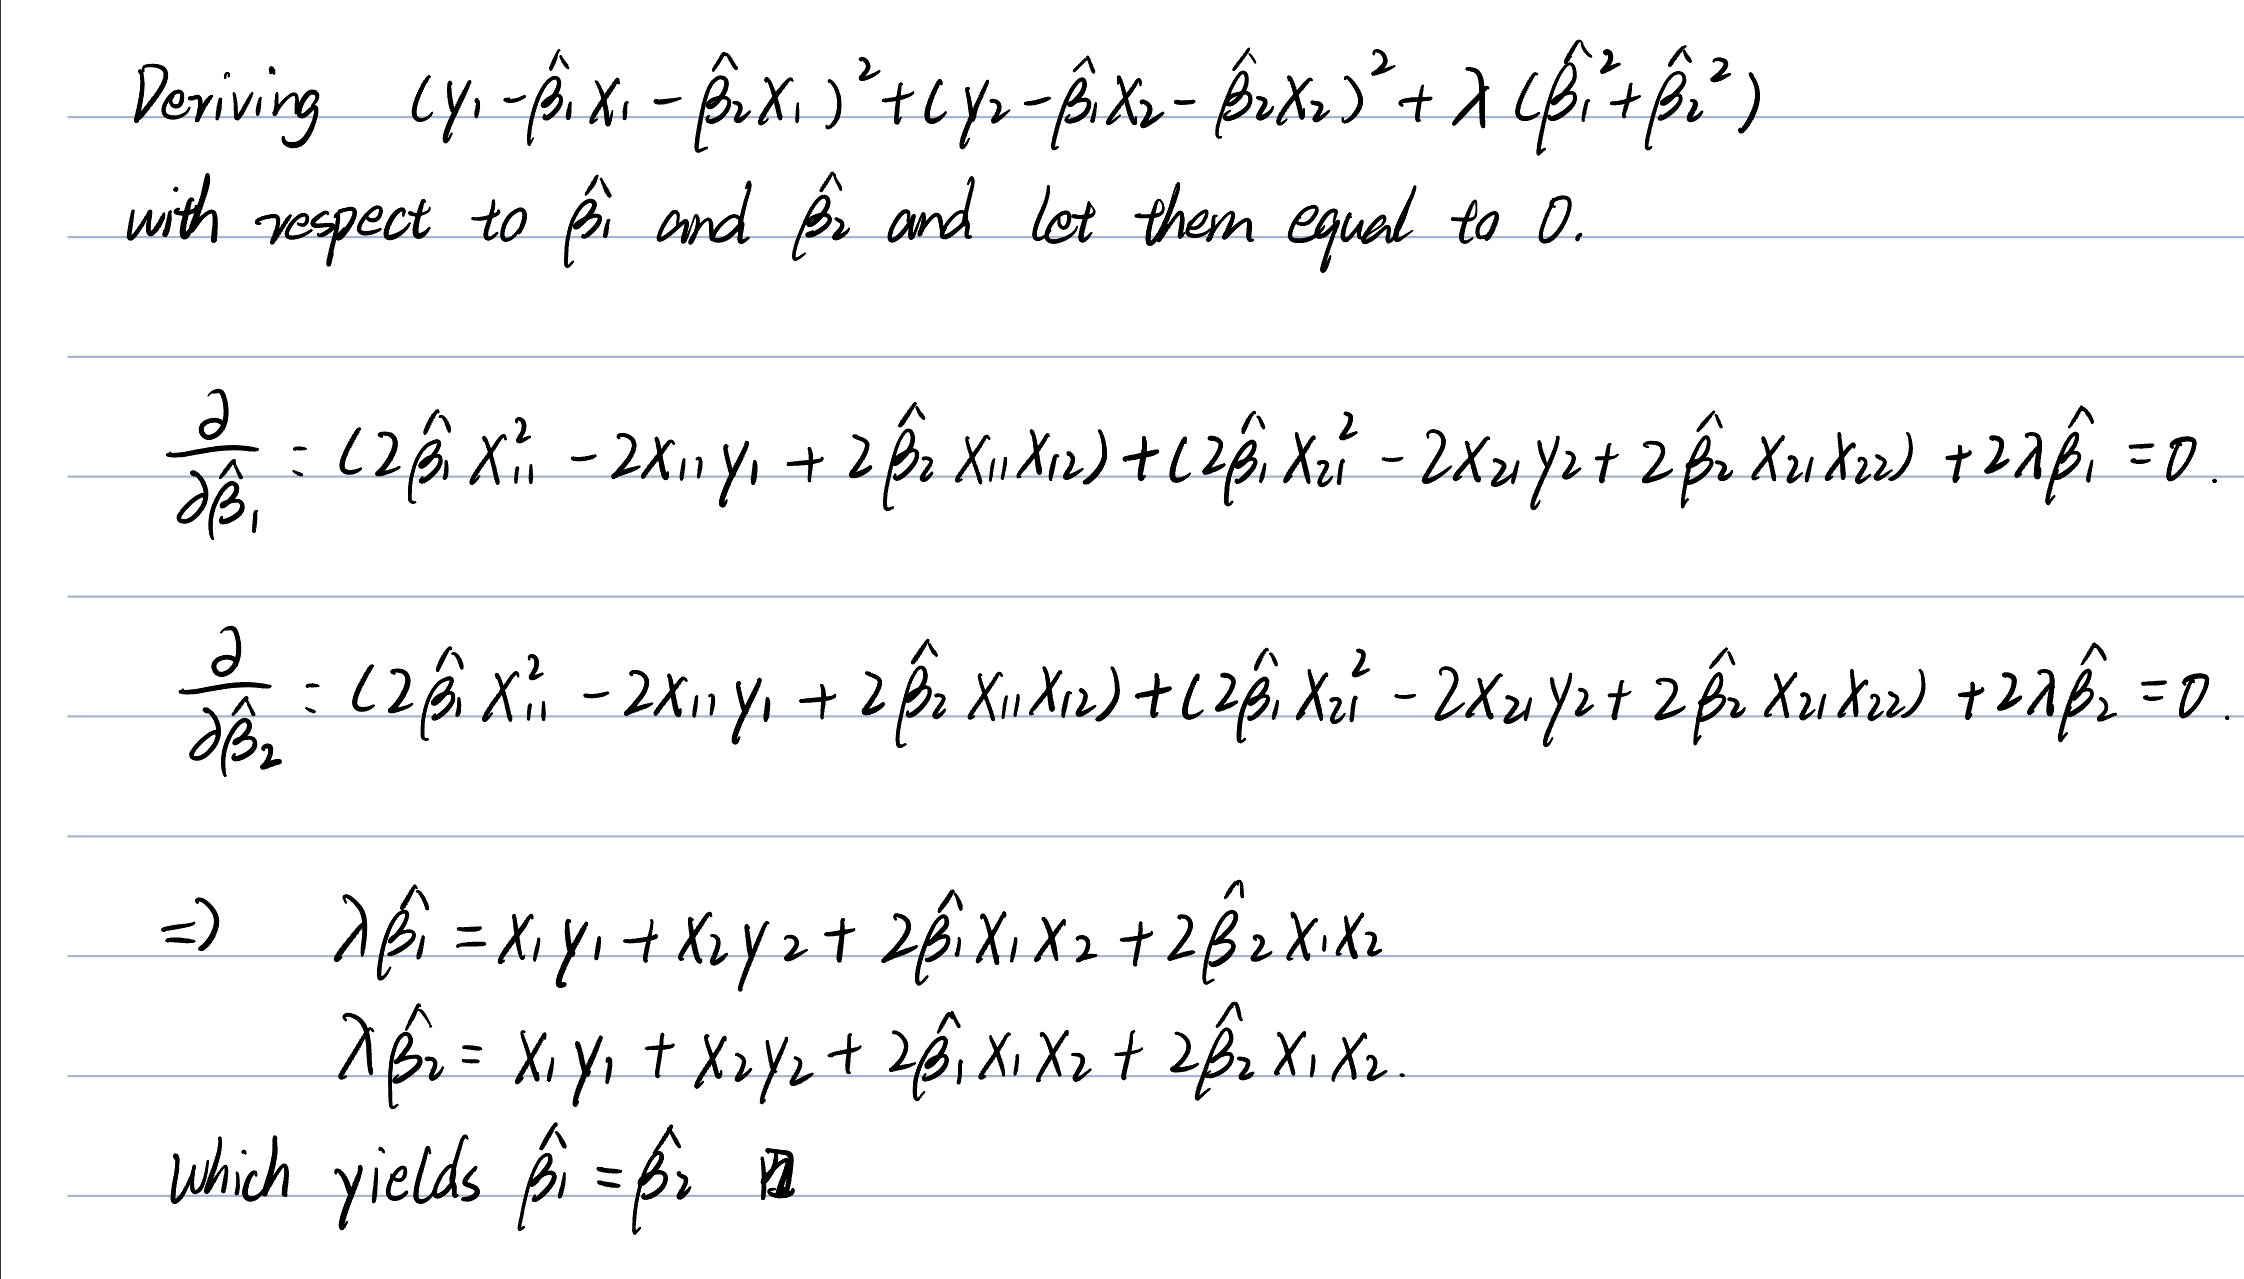
\includegraphics{IMG_274FE6CD7017-1.jpeg}
\end{center}

\textbf{(c)}\\
The Lasso regression optimization problem is:\\
\[
\sum_{i=1}^{n} \left( y_i - \beta_0 - \sum_{j=1}^{p} \beta_j x_{ij} \right)^2 + \lambda \sum_{j=1}^{p} |\beta_j|
\] Given \(n = 2, p = 2\), the predictor matrix is:\\
\[
X = \begin{bmatrix} x_{11} & x_{12} \\ x_{21} & x_{22} \end{bmatrix}
\] Lasso regression estimates coefficients by minimizing:\\
\[
\sum_{i=1}^{2} \left( y_i - \beta_0 - \beta_1 x_{i1} - \beta_2 x_{i2} \right)^2 + \lambda (|\beta_1| + |\beta_2|)
\] With \(\beta_0 = 0\), this simplifies to:\\
\[
(y_1 - \beta_1 x_{11} - \beta_2 x_{12})^2 + (y_2 - \beta_1 x_{21} - \beta_2 x_{22})^2 + \lambda (|\beta_1| + |\beta_2|)
\] Since predictors are perfectly correlated:\\
\[
2(y_1 - \hat{\beta}_1 x_{11} - \hat{\beta}_2 x_{11})^2 + \lambda (|\beta_1| + |\beta_2|)
\] \textbf{(d)}\\
Lasso solutions are not unique because the constraint (
\textbar{}\hat{\beta}\_1\textbar{} + \textbar{}\hat{\beta}\_2\textbar{}
\leq s ) forms a diamond-shaped region centered at ( (0,0) ). The
optimization process seeks to minimize the squared error subject to this
constraint.

The objective function: \[
\sum_{i=1}^{n} \left( y_i - \beta_0 - \sum_{j=1}^{p} \beta_j x_{ij} \right)^2 + \lambda \sum_{j=1}^{p} |\beta_j|
\]

Given the specific setting, the minimization reduces to: \[
\min \left[ 2(y_1 - (\hat{\beta}_1 + \hat{\beta}_2) x_{11}) \right]
\] Since the Lasso constraint enforces (
\textbar{}\hat{\beta}\_1\textbar{} + \textbar{}\hat{\beta}\_2\textbar{}
= s ), this defines a \textbf{line segment} on the boundary of the
diamond. The final solution is \textbf{not unique}, as any point on this
edge satisfies the optimization.

We can illustrate this by plotting the feasible region and the solution
path.

\begin{center}
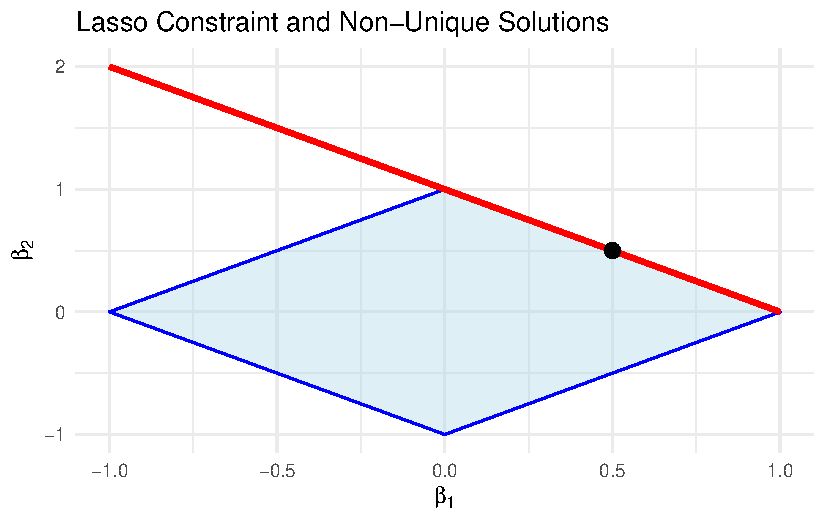
\includegraphics{hw3_files/figure-pdf/unnamed-chunk-13-1.pdf}
\end{center}

\subsection{ISL Exercise 6.6.11
(30pts)}\label{isl-exercise-6.6.11-30pts}

You must follow the
\href{https://ucla-biostat-212a.github.io/2024winter/slides/06-modelselection/workflow_lasso.html}{typical
machine learning paradigm} to compare \emph{at least} 3 methods: least
squares, lasso, and ridge. Report final results as

\begin{longtable}[]{@{}cccc@{}}
\toprule\noalign{}
Method & CV RMSE & Test RMSE & \\
\midrule\noalign{}
\endhead
\bottomrule\noalign{}
\endlastfoot
LS & & & \\
Ridge & & & \\
Lasso & & & \\
\ldots{} & & & \\
\end{longtable}

\begin{Shaded}
\begin{Highlighting}[]
\FunctionTok{library}\NormalTok{(MASS) }
\FunctionTok{library}\NormalTok{(leaps)   }
\FunctionTok{library}\NormalTok{(glmnet) }
\FunctionTok{library}\NormalTok{(pls)    }

\FunctionTok{data}\NormalTok{(Boston)}
\FunctionTok{set.seed}\NormalTok{(}\DecValTok{1}\NormalTok{)}

\NormalTok{train\_index }\OtherTok{=} \FunctionTok{sample}\NormalTok{(}\DecValTok{1}\SpecialCharTok{:}\FunctionTok{nrow}\NormalTok{(Boston), }\FunctionTok{nrow}\NormalTok{(Boston) }\SpecialCharTok{*} \FloatTok{0.8}\NormalTok{)}
\NormalTok{train\_data }\OtherTok{=}\NormalTok{ Boston[train\_index, ]}
\NormalTok{test\_data }\OtherTok{=}\NormalTok{ Boston[}\SpecialCharTok{{-}}\NormalTok{train\_index, ]}

\NormalTok{x\_train }\OtherTok{=} \FunctionTok{model.matrix}\NormalTok{(crim }\SpecialCharTok{\textasciitilde{}}\NormalTok{ ., train\_data)[, }\SpecialCharTok{{-}}\DecValTok{1}\NormalTok{]}
\NormalTok{y\_train }\OtherTok{=}\NormalTok{ train\_data}\SpecialCharTok{$}\NormalTok{crim}

\NormalTok{x\_test }\OtherTok{=} \FunctionTok{model.matrix}\NormalTok{(crim }\SpecialCharTok{\textasciitilde{}}\NormalTok{ ., test\_data)[, }\SpecialCharTok{{-}}\DecValTok{1}\NormalTok{]}
\NormalTok{y\_test }\OtherTok{=}\NormalTok{ test\_data}\SpecialCharTok{$}\NormalTok{crim}
\end{Highlighting}
\end{Shaded}

\begin{Shaded}
\begin{Highlighting}[]
\CommentTok{\# {-}{-}{-}{-}{-}{-}{-}{-}{-}{-}{-}{-}{-}{-}{-}{-}{-}{-}{-}{-}{-}{-}{-}{-}{-}{-}}
\CommentTok{\# Step 1: CV RMSE}
\CommentTok{\# {-}{-}{-}{-}{-}{-}{-}{-}{-}{-}{-}{-}{-}{-}{-}{-}{-}{-}{-}{-}{-}{-}{-}{-}{-}{-}}
\NormalTok{predict.regsubsets }\OtherTok{=} \ControlFlowTok{function}\NormalTok{(object, newdata, id, ...) \{}
\NormalTok{    form }\OtherTok{=} \FunctionTok{as.formula}\NormalTok{(object}\SpecialCharTok{$}\NormalTok{call[[}\DecValTok{2}\NormalTok{]])}
\NormalTok{    mat }\OtherTok{=} \FunctionTok{model.matrix}\NormalTok{(form, newdata)}
\NormalTok{    coefi }\OtherTok{=} \FunctionTok{coef}\NormalTok{(object, }\AttributeTok{id =}\NormalTok{ id)}
\NormalTok{    xvars }\OtherTok{=} \FunctionTok{names}\NormalTok{(coefi)}
\NormalTok{    mat[, xvars] }\SpecialCharTok{\%*\%}\NormalTok{ coefi}
\NormalTok{\}}

\NormalTok{k }\OtherTok{=} \DecValTok{10}
\NormalTok{folds }\OtherTok{=} \FunctionTok{sample}\NormalTok{(}\DecValTok{1}\SpecialCharTok{:}\NormalTok{k, }\FunctionTok{nrow}\NormalTok{(Boston), }\AttributeTok{replace =} \ConstantTok{TRUE}\NormalTok{)}
\NormalTok{cv.errors }\OtherTok{=} \FunctionTok{matrix}\NormalTok{(}\ConstantTok{NA}\NormalTok{, k, }\DecValTok{13}\NormalTok{, }\AttributeTok{dimnames =} \FunctionTok{list}\NormalTok{(}\ConstantTok{NULL}\NormalTok{, }\FunctionTok{paste}\NormalTok{(}\DecValTok{1}\SpecialCharTok{:}\DecValTok{13}\NormalTok{)))}
\ControlFlowTok{for}\NormalTok{ (j }\ControlFlowTok{in} \DecValTok{1}\SpecialCharTok{:}\NormalTok{k) \{}
\NormalTok{    best.fit }\OtherTok{=} \FunctionTok{regsubsets}\NormalTok{(crim }\SpecialCharTok{\textasciitilde{}}\NormalTok{ ., }\AttributeTok{data =}\NormalTok{ Boston[folds }\SpecialCharTok{!=}\NormalTok{ j, ], }\AttributeTok{nvmax =} \DecValTok{13}\NormalTok{)}
    \ControlFlowTok{for}\NormalTok{ (i }\ControlFlowTok{in} \DecValTok{1}\SpecialCharTok{:}\DecValTok{13}\NormalTok{) \{}
\NormalTok{        pred }\OtherTok{=} \FunctionTok{predict}\NormalTok{(best.fit, Boston[folds }\SpecialCharTok{==}\NormalTok{ j, ], }\AttributeTok{id =}\NormalTok{ i)}
\NormalTok{        cv.errors[j, i] }\OtherTok{=} \FunctionTok{mean}\NormalTok{((Boston}\SpecialCharTok{$}\NormalTok{crim[folds }\SpecialCharTok{==}\NormalTok{ j] }\SpecialCharTok{{-}}\NormalTok{ pred)}\SpecialCharTok{\^{}}\DecValTok{2}\NormalTok{)}
\NormalTok{    \}}
\NormalTok{\}}
\NormalTok{mean.cv.errors }\OtherTok{=} \FunctionTok{apply}\NormalTok{(cv.errors, }\DecValTok{2}\NormalTok{, mean)}
\FunctionTok{plot}\NormalTok{(mean.cv.errors, }\AttributeTok{type =} \StringTok{"b"}\NormalTok{, }\AttributeTok{xlab =} \StringTok{"Number of variables"}\NormalTok{, }\AttributeTok{ylab =} \StringTok{"CV error"}\NormalTok{)}
\end{Highlighting}
\end{Shaded}

\begin{center}
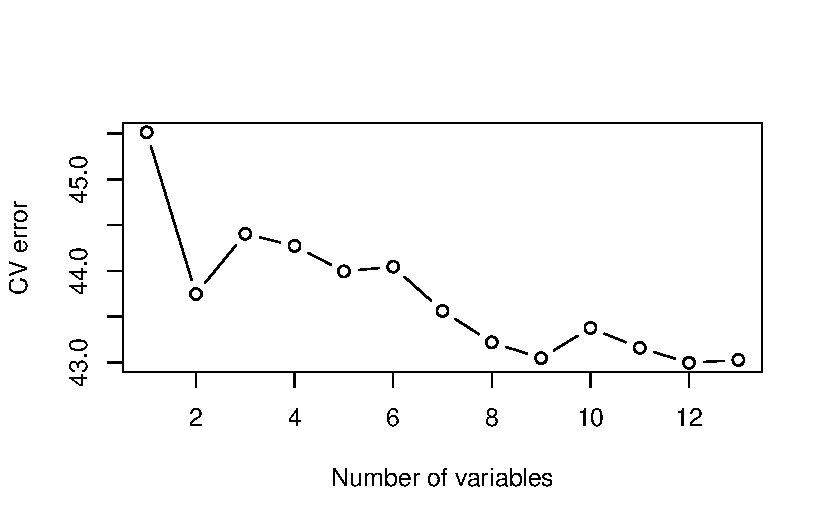
\includegraphics{hw3_files/figure-pdf/unnamed-chunk-15-1.pdf}
\end{center}

\begin{Shaded}
\begin{Highlighting}[]
\CommentTok{\# min CV RMSE}
\FunctionTok{min}\NormalTok{(mean.cv.errors)}
\end{Highlighting}
\end{Shaded}

\begin{verbatim}
[1] 42.99579
\end{verbatim}

\begin{Shaded}
\begin{Highlighting}[]
\NormalTok{regfit.best }\OtherTok{=} \FunctionTok{regsubsets}\NormalTok{(crim}\SpecialCharTok{\textasciitilde{}}\NormalTok{., }\AttributeTok{data=}\NormalTok{Boston, }\AttributeTok{nvmax=}\DecValTok{13}\NormalTok{)}
\FunctionTok{coef}\NormalTok{(regfit.best, }\DecValTok{12}\NormalTok{)}
\end{Highlighting}
\end{Shaded}

\begin{verbatim}
  (Intercept)            zn         indus          chas           nox 
 16.985713928   0.044673247  -0.063848469  -0.744367726 -10.202169211 
           rm           dis           rad           tax       ptratio 
  0.439588002  -0.993556631   0.587660185  -0.003767546  -0.269948860 
        black         lstat          medv 
 -0.007518904   0.128120290  -0.198877768 
\end{verbatim}

\begin{Shaded}
\begin{Highlighting}[]
\CommentTok{\# {-}{-}{-}{-}{-}{-}{-}{-}{-}{-}{-}{-}{-}{-}{-}{-}{-}{-}{-}{-}{-}{-}{-}{-}{-}{-}}
\CommentTok{\# Step 2: Lasso}
\CommentTok{\# {-}{-}{-}{-}{-}{-}{-}{-}{-}{-}{-}{-}{-}{-}{-}{-}{-}{-}{-}{-}{-}{-}{-}{-}{-}{-}}
\NormalTok{lasso\_model }\OtherTok{=} \FunctionTok{cv.glmnet}\NormalTok{(x\_train, y\_train, }\AttributeTok{alpha =} \DecValTok{1}\NormalTok{, }\AttributeTok{type.measure =} \StringTok{"mse"}\NormalTok{)}

\CommentTok{\# CV RMSE}
\NormalTok{lasso\_cv\_rmse }\OtherTok{=} \FunctionTok{sqrt}\NormalTok{(}\FunctionTok{min}\NormalTok{(lasso\_model}\SpecialCharTok{$}\NormalTok{cvm))}

\CommentTok{\# Test RMSE}
\NormalTok{lasso\_pred }\OtherTok{=} \FunctionTok{predict}\NormalTok{(lasso\_model, }\AttributeTok{s =}\NormalTok{ lasso\_model}\SpecialCharTok{$}\NormalTok{lambda.min, }\AttributeTok{newx =}\NormalTok{ x\_test)}
\NormalTok{lasso\_test\_rmse }\OtherTok{=} \FunctionTok{sqrt}\NormalTok{(}\FunctionTok{mean}\NormalTok{((y\_test }\SpecialCharTok{{-}}\NormalTok{ lasso\_pred)}\SpecialCharTok{\^{}}\DecValTok{2}\NormalTok{))}

\FunctionTok{plot}\NormalTok{(lasso\_model)}
\end{Highlighting}
\end{Shaded}

\begin{center}
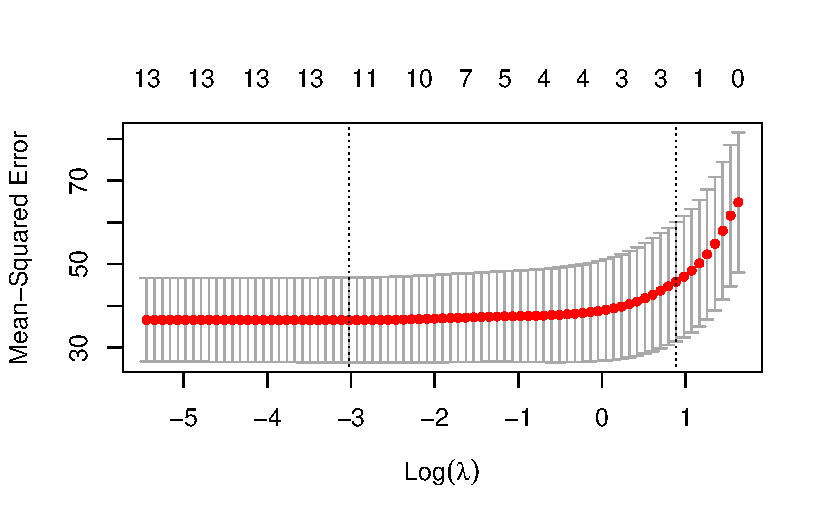
\includegraphics{hw3_files/figure-pdf/unnamed-chunk-18-1.pdf}
\end{center}

\begin{Shaded}
\begin{Highlighting}[]
\CommentTok{\# {-}{-}{-}{-}{-}{-}{-}{-}{-}{-}{-}{-}{-}{-}{-}{-}{-}{-}{-}{-}{-}{-}{-}{-}{-}{-}}
\CommentTok{\# Step 3: Ridge}
\CommentTok{\# {-}{-}{-}{-}{-}{-}{-}{-}{-}{-}{-}{-}{-}{-}{-}{-}{-}{-}{-}{-}{-}{-}{-}{-}{-}{-}}
\NormalTok{ridge\_model }\OtherTok{=} \FunctionTok{cv.glmnet}\NormalTok{(x\_train, y\_train, }\AttributeTok{alpha =} \DecValTok{0}\NormalTok{, }\AttributeTok{type.measure =} \StringTok{"mse"}\NormalTok{)}

\CommentTok{\# CV RMSE}
\NormalTok{ridge\_cv\_rmse }\OtherTok{=} \FunctionTok{sqrt}\NormalTok{(}\FunctionTok{min}\NormalTok{(ridge\_model}\SpecialCharTok{$}\NormalTok{cvm))}

\CommentTok{\# Test RMSE}
\NormalTok{ridge\_pred }\OtherTok{=} \FunctionTok{predict}\NormalTok{(ridge\_model, }\AttributeTok{s =}\NormalTok{ ridge\_model}\SpecialCharTok{$}\NormalTok{lambda.min, }\AttributeTok{newx =}\NormalTok{ x\_test)}
\NormalTok{ridge\_test\_rmse }\OtherTok{=} \FunctionTok{sqrt}\NormalTok{(}\FunctionTok{mean}\NormalTok{((y\_test }\SpecialCharTok{{-}}\NormalTok{ ridge\_pred)}\SpecialCharTok{\^{}}\DecValTok{2}\NormalTok{))}
\end{Highlighting}
\end{Shaded}

\begin{Shaded}
\begin{Highlighting}[]
\CommentTok{\# {-}{-}{-}{-}{-}{-}{-}{-}{-}{-}{-}{-}{-}{-}{-}{-}{-}{-}{-}{-}{-}{-}{-}{-}{-}{-}}
\CommentTok{\# Step 4: Least Squares (LS)}
\CommentTok{\# {-}{-}{-}{-}{-}{-}{-}{-}{-}{-}{-}{-}{-}{-}{-}{-}{-}{-}{-}{-}{-}{-}{-}{-}{-}{-}}
\NormalTok{ls\_model }\OtherTok{=} \FunctionTok{lm}\NormalTok{(crim }\SpecialCharTok{\textasciitilde{}}\NormalTok{ ., }\AttributeTok{data =}\NormalTok{ train\_data)}

\CommentTok{\# CV RMSE}
\NormalTok{ls\_cv\_rmse }\OtherTok{=} \FunctionTok{sqrt}\NormalTok{(}\FunctionTok{mean}\NormalTok{(ls\_model}\SpecialCharTok{$}\NormalTok{residuals}\SpecialCharTok{\^{}}\DecValTok{2}\NormalTok{))}

\CommentTok{\# Test RMSE}
\NormalTok{ls\_pred }\OtherTok{=} \FunctionTok{predict}\NormalTok{(ls\_model, }\AttributeTok{newdata =}\NormalTok{ test\_data)}
\NormalTok{ls\_test\_rmse }\OtherTok{=} \FunctionTok{sqrt}\NormalTok{(}\FunctionTok{mean}\NormalTok{((y\_test }\SpecialCharTok{{-}}\NormalTok{ ls\_pred)}\SpecialCharTok{\^{}}\DecValTok{2}\NormalTok{))}
\end{Highlighting}
\end{Shaded}

\begin{Shaded}
\begin{Highlighting}[]
\CommentTok{\# {-}{-}{-}{-}{-}{-}{-}{-}{-}{-}{-}{-}{-}{-}{-}{-}{-}{-}{-}{-}{-}{-}{-}{-}{-}{-}}
\CommentTok{\# Step 5: results}
\CommentTok{\# {-}{-}{-}{-}{-}{-}{-}{-}{-}{-}{-}{-}{-}{-}{-}{-}{-}{-}{-}{-}{-}{-}{-}{-}{-}{-}}
\NormalTok{results }\OtherTok{\textless{}{-}} \FunctionTok{data.frame}\NormalTok{(}
  \AttributeTok{Method =} \FunctionTok{c}\NormalTok{(}\StringTok{"Least Squares"}\NormalTok{, }\StringTok{"Ridge"}\NormalTok{, }\StringTok{"Lasso"}\NormalTok{),}
  \AttributeTok{CV\_RMSE =} \FunctionTok{c}\NormalTok{(ls\_cv\_rmse, ridge\_cv\_rmse, lasso\_cv\_rmse),}
  \AttributeTok{Test\_RMSE =} \FunctionTok{c}\NormalTok{(ls\_test\_rmse, ridge\_test\_rmse, lasso\_test\_rmse)}
\NormalTok{)}

\FunctionTok{print}\NormalTok{(results)}
\end{Highlighting}
\end{Shaded}

\begin{verbatim}
         Method  CV_RMSE Test_RMSE
1 Least Squares 5.801427  8.317917
2         Ridge 6.148486  8.408933
3         Lasso 6.049605  8.345760
\end{verbatim}

\subsection{Bonus question (20pts)}\label{bonus-question-20pts}

Consider a linear regression, fit by least squares to a set of training
data \((x_1, y_1), \ldots, (x_N,  y_N)\) drawn at random from a
population. Let \(\hat \beta\) be the least squares estimate. Suppose we
have some test data
\((\tilde{x}_1, \tilde{y}_1), \ldots, (\tilde{x}_M, \tilde{y}_M)\) drawn
at random from the same population as the training data. If
\(R_{\text{train}}(\beta) = \frac{1}{N} \sum_{i=1}^N (y_i - \beta^T x_i)^2\)
and
\(R_{\text{test}}(\beta) = \frac{1}{M} \sum_{i=1}^M (\tilde{y}_i - \beta^T \tilde{x}_i)^2\).
Show that \[
\operatorname{E}[R_{\text{train}}(\hat{\beta})] < \operatorname{E}[R_{\text{test}}(\hat{\beta})].
\]

\begin{center}
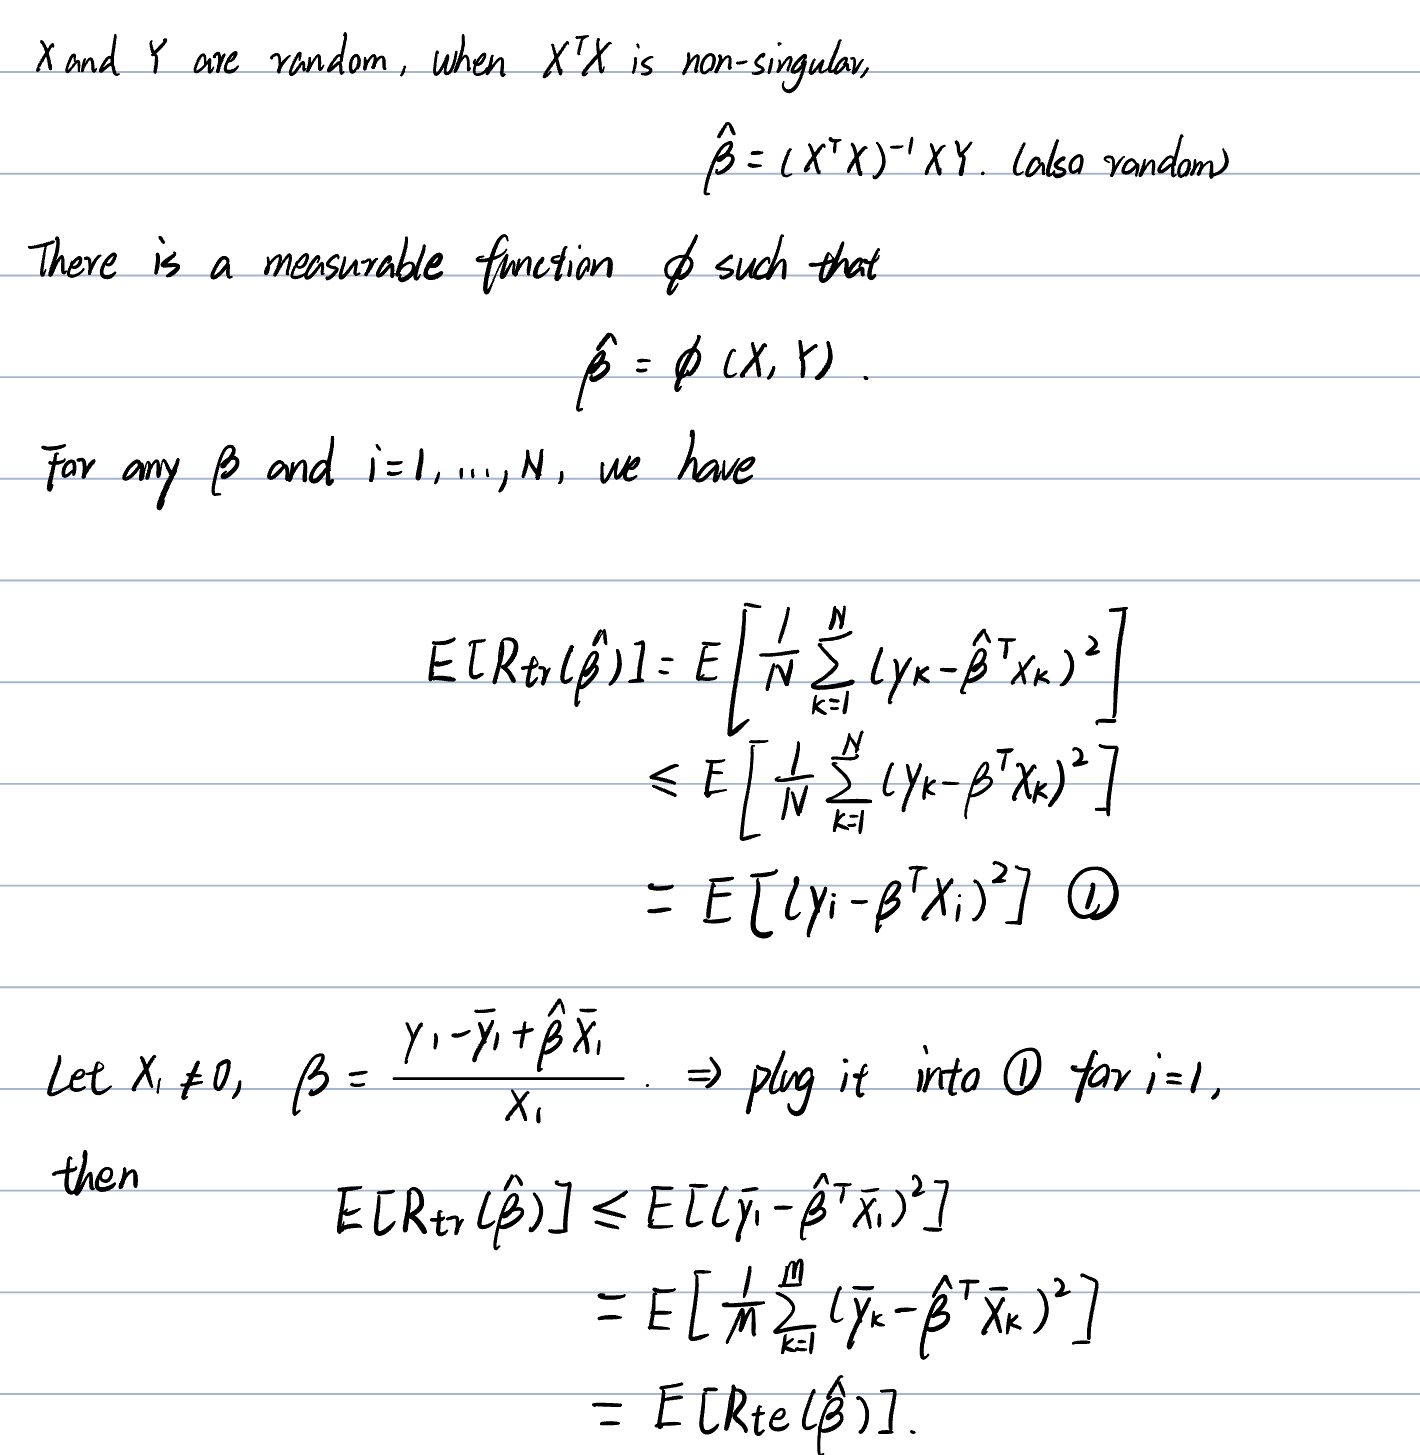
\includegraphics{IMG_3CF00996EB9E-1.jpeg}
\end{center}




\end{document}
